\chapter{Hardware\label{chap:Hardware}}

%Introduction ===============================================================================
\section{Introduction\label{Section:Hardware:Introduction}}

Evidence presented in Australian courtrooms is increasing in technical complexity continually. This increase in the technical complexity of evidence is largely due to avdancements in scientific evidence collection techniques. As a result of this increasing complexity of evidence the requirements for presentation for this evidence has also become far more complex. To date, the solution to the display needs for evidence is approached in a adhock way based on the singular type of evidence being presented. This has resulted in a patchwork of technologies being used with little or no integration between the various technologies used for presentation, and very little standardisation of technologies between the different Courts, and between different courtrooms within a Court. 

Introduction of an integrated evidence display system for Australian courtrooms is very complex. Not only does the software need the correct functioanlity, and excellent usability (discussed in  \refChap{chap:Software}), but it also needs the correct choice of hardware. The rapid adoption of tablet technology seen not only in the Australian population, but also within the Australian judiciary \citep{Heerboth2013} can be seen as a very real opportunity to advance evidence presentation by using this technology.

For the introduction of new evidence display technology it is essential to understand how the stakeholders will perceive its introduction. The Technology Acceptance Model (TAM) identified two key areas for technology acceptance. They are precieved usefulness of the technology, and the percieved ease of use of the technology. To accurately guage these two areas for evidence display technology the involvement and input from all members of the courtroom is critical. 

This chapter will discuss two studies conducted with key stakeholders designed to guage the usefullness, and the ease of use of tablet technology for evidence presentation purposes. The first study was conducted as a future technology workshop, allowing candidates to operate iPads for the purpose of displaying evidence. The second study, informed by the results of the first study, was a Moot Court session using centralised control and push technology to allow the candidates to participate in a real trial situation. Each study was conducted twice with different canidiates.

The studies will be examined in detail, results analysed, and recommendations made.  





% Studies & Methodologies====================================================================
\section{Studies \& Methodologies\label{Hardware:Studies and Methodologies}}








% Study 1 ===================================================================================
\section{Study 1\label{Hardware:Study 1}}
\subsection{Study Design}
This study was conducted at the Tribunal of Tomorrow conference 2012, over two sessions, with approximately 80 participants. Participants included judges, barristers, lawyers, and court administrators, and were drawn from all levels of Courts and Tribunals in Australia.
Participants were supplied with iPads that had the Exhibit A application installed, and digital evidence installed via Dropbox. 
The choice of Exhibit A as the evidence display application for this study was informed by the prior study into evidence display appliccations discussed in \refChap{chap:Software}, primarilary due to the applications ease of use and affordability.
Participants that were inexperienced in the use of iPads were briefed on the iPads basic functionality and demonstrated the control gestures for common operations such as zooming and scrolling.
A courtroom environment was created where participants played the roles  of a presiding judge and jurors receiving evidence, and wittnesses interacting with the evidence. Participants were rotated through each of these roles so as to experience the demonstration from each viewpoint. The participants were led through a narrated case based on an actual wrongful death case that took place in Canada. The evidence used was the actual evidence from the Canadian case, and the narrated script was closely based on the transcript of the Canadian case.
The evidence used for this study was primarilary in PDF format, and also included scanned documents, images and video. Participants were required to navigate to and view each piece of evidence, this often involving some manipulation of the evidence. This required manipulation included navigating within a document, zooming, redacting, highlighting, annotating, paragraph extraction, and white board drawing.
Support staff were located throughout the room to ensure that participants followed the path of evidence, however free roaming of the evidence was also permitted. Participants were required to save any evidence file that they had modified through any form of manipulation.
On conclusion of the demonstration a forum was held with participants, and participants were asked to complete a comprehensive survey about their experience. The survey was designed to identify the demographic of the participant, their attitude towards technology, the strengths and weaknesses of the application, and their percieved needs and priorities to be considered when designing an evidence presentation system for Australian courtrooms.

\subsection{Results}
\subsubsection{Participant Demographic and General Computer Familiarity}
The vast majority (87\%) of particcipants where experience with or involved in court processes, the remaininf 13\% of participants were non-judicial support staff. All participants stated that they used computers for their work, with the majority having experience using tablets for tasks including email, document preperation, looking up legislation, and other internet searching throught a browser.
Overall the participant group can be considered computer literate.

\subsubsection{Response to Coutroom Evidence Simulation}
This section will initalyy examine the general response of participants to using Exhibit A for the Moot Court demonstration, and will then discuss in detail the identified areas of concern raised by the participants.
88\% of participants indicated a high level of ease operating the Exhibit A Case management functionality which includes remaning, accessing, closing, amending, and appending files and folders within an existing case. 

%\begin{center}
%\begin{table}[htbp]
    


%\small
%\centering

%\singlespace

%\begin{tabular}{ c c } 

% insert Graphics


\begin{figure}[h] \centering
% \begin{subfigure}[]{0.4\textwidth}
% 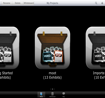
\includegraphics[height=1.2in]{Exhibit_A_Cases}
% \caption{Exhibit A - Cases directory}
% \label{fig:exhibit_a_cases_Directory}
% \end{subfigure}
\subfloat [Exhibit A - Cases directory]
{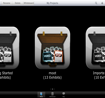
\includegraphics{Exhibit_A_Cases}
\label{fig:exhibit_a_cases_Directory}}

%     \begin{subfigure}[t]{0.4\textwidth}
% 
%         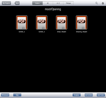
\includegraphics[height=1.2in]{Exhibit_A_Exhibits}
%         \caption{Exhibit A - Exhibits folder}
%         \label{Exhibit_A_Exhibits}
%     \end{subfigure}%
\hspace{0.5cm}
\subfloat[Exhibit_A_Exhibits]{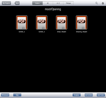
\includegraphics{Exhibit_A_Exhibits}\label{Exhibit_A_Exhibits}}

\end{figure}
%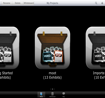
\includegraphics[width=0.4\textwidth]{Exhibit_A_Cases}
%\caption{Exhibit A - Cases directory}



%&

% \begin{figure}[h]
% 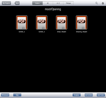
\includegraphics[width=0.4\textwidth]{Exhibit_A_Exhibits}
% \caption{Exhibit A - Exhibits folder}
% \label{fig:exhibit_a_exhibits_folder}
% \end{figure}

%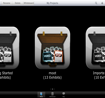
\includegraphics{Exhibit_A_Cases} & 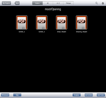
\includegraphics{Exhibit_A_Exhibits}\\

%\end{tabular}
%\end{table}
%\end{center}

% \begin{minipage}[c]{0.5\textwidth}
%    \begin{figure}[h]
%       \centering
%       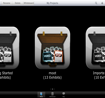
\includegraphics[height=1in]{Exhibit_A_Cases}
%       \caption{Example LaTeX Figure} 
%       \label{fig:NASA_Logo2}
%    \end{figure}
% \end{minipage}%
% \begin{minipage}[c]{0.5\textwidth}
%    \begin{figure}[h]
%       \centering
%       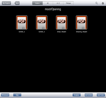
\includegraphics[height=1in]{Exhibit_A_Exhibits}
%       \caption{Example LaTeX Figure} 
%       \label{fig:Orion_Logo2}
%    \end{figure}
% \end{minipage}


Graphics manipulation functionality was responded to favourably by 88\% of the participants. This functionality includes highlighting, zooming, drawing on whiteboard, enlargement of image section, selecting drawing tools, erasing, and using the undo option. It was generally felt that that this functionality offered the user the ability to manipulate the user interface to best suit the user in preparing the material for further consideration.
It was observed during this study that the impact of the graphic manipulation functionality greatly impressed many of the participants. Participants repeatedly refered to it's contribution to the enhancement of evidence presentation throughout the evidence presentation and in the post case forum.

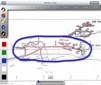
\includegraphics{Exhibit_A_Drawing_Tools}

Participants response to the multimedia functionality was also very positive with 88\% of participants responding favourably. This functionality included opening video files, full screen display, and video controls.  

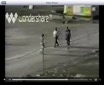
\includegraphics{Exhibit_A_Video_Controls}

Manipulation of text in a PDF document was also highly rated by participants, with 80\% responding favourably for the functionality of highlighting using a pen, block highlighting, redacting (censoring), magnification to call out lines, and saving the edited file. It is noted that there were some issues identified with these functionalities which will be discussed in the following section.

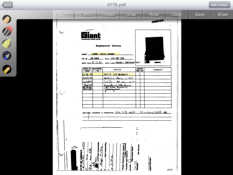
\includegraphics{Exhibit_A_PDF_Highlight}
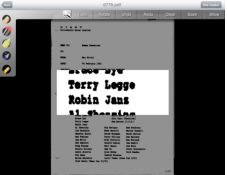
\includegraphics{Exhibit_A_PDF_Magnify}

Participants were less impressed with the cross Case management functionality, which includes file transfer between Cases, file duplication file searching, and file downloading from Dropbox. Only 50\% of participants found this functionality satisfactory.

\subsection{Issues Identified and Suggested Solutions}
Even though the large majority of participants in the Moot Court viewed the general functionality of Exhibit A as accepatble, managable, and innovative, the following were identified.
The following tables (\refTable{tab:Issues_General_Operation} - \refTable{tab:Issues_File_Management}) show issues with Exhibit A using the severity scale of 1 for No Real Concern, up to 5 for Critical \citep{Nielsen1990}.

% General Operation Table=========================================
\begin{center}
\begin{table}[htbp]
\label{tab:Issues_General_Operation}
  \centering
  \caption{General Operation}
    \begin{tabular}{|p{0.40\textwidth}|c|p{0.40\textwidth}|}
    \hline
    \rowcolor{lightgrey}\multicolumn{3}{|l|}{General Operation} \\
    \hline
    \textbf{Areas and Issues of Concern} & \textbf{Sev 0-5} & \textbf{Suggested Solution}\\
    \hline
    iPad working area too small & 2 & Alternative larger size sceen tablet device\\
    \hline
    Difficult to master quickly & 1 & Training in package required pre-trial\\
    \hline
   Scrolling can be too sensative and unstable causing system failure. & 5 & Use of arrows more reliable and controlable. Requires urgent debugging.\\
   \hline
   Finger based manipulation required too high a level of dexterity, especially for underlining. & 4 & Develope snap lock option, use block highlighting as much as possible.\\
   \hline
   Editing tools remail selected after use. & 2 & Redesign with editing tools auto deselecting after use.\\
   \hline
   
\end{tabular}
\end{table}
\end{center}

%Graphics and Multimedia Table===================================================
\begin{center}
\begin{table}[htbp]
\label{tab:Issues_Grapgics_and_Multimedia}
  \centering
  \caption{Graphics and Multimedia}
    \begin{tabular}{|p{0.40\textwidth}|c|p{0.40\textwidth}|}
    \hline
    \rowcolor{lightgrey}\multicolumn{3}{|l|}{Graphics and Multimedia} \\
    \hline
    \textbf{Areas and Issues of Concern} & \textbf{Sev 0-5} & \textbf{Suggested Solution}\\
    \hline
    Difficult to find tool bar for drawing & 2 & Training and increas visibility of tool bar\\
    \hline
    Projection, even though it works for video it does not for the other evidence elements & 3 & General restriction imposed by iPad. alternative Windows tablet may offer more flexability.\\
    \hline
\end{tabular}
\end{table}
\end{center}

%Document Manipulation Table==============================================================================
\begin{center}
\begin{table}[htbp]
\label{tab:Issues_Document_Manipulation}
  \centering
  \caption{Document Manipulation}
    \begin{tabular}{|p{0.40\textwidth}|c|p{0.40\textwidth}|}
    \hline
    \rowcolor{lightgrey}\multicolumn{3}{|l|}{Document manipulation} \\
    \hline
    \textbf{Areas and Issues of Concern} & \textbf{Sev 0-4} & \textbf{Suggested Solution}\\
    \hline
    Highlighting not bright enough. & 2 & Redesign to offer stronger highlighting tool\\
    \hline
    Saved edited document destination is not consistent. & 4 & Redesign with consistant save destination.\\
    \hline
   Saved edited documents not saved in their entirity. Only currently visible page is saved. & 5 & Redesign with complete document saving.\\
   \hline
   Functional icons confusing, eg. ``Search'' is represented as a magnifying glass. & 2 & Redesign with icins offering strong affordance.\\
   \hline
\end{tabular}
\end{table}
\end{center}

%File Management Table==============================================
\begin{center}
\begin{table}[htbp]
\label{tab:Issues_File_Management}
  \centering
  \caption{File Management}
    \begin{tabular}{|p{0.40\textwidth}|c|p{0.40\textwidth}|}
    \hline
    \rowcolor{lightgrey}\multicolumn{3}{|l|}{File Management} \\
    \hline
    \textbf{Areas and Issues of Concern} & \textbf{Sev 0-4} & \textbf{Suggested Solution}\\
    \hline
    Inconsistant termanology, eg. Cases / Files used interchangeably. & 2 & Redevelop with consistant terminology\\
    \hline
    Improve ``Search'' option, difficult to find evidence files, inconsistant destinations. & 4 & Redesign with coherent file management order, with Search functionality consistant to it. Windows tablet option offers stronger alternative.\\
    \hline
    Offer more warnings with delete command. & 4 & Redesign with more warnings, and offer a recovery option to retreive deleted files.\\
   \hline
   Difficult to add exhibits. & 1 & Training required.\\
   \hline
   No levels of ``undo'', just the one step back function. & 4 & Redesign to offer incremental undo functionality.\\
   \hline
   File icon size does not allow larger folders to be properly displayed. & 2 & Redesign with smaller file icons, possible thumbnails for expansion if required.\\
   \hline
   Files are displayed in order of creation. & 2 & Redesign for files to be listed according to a user preference.\\
   \hline
   
\end{tabular}
\end{table}
\end{center}
\subsection{Analysis and Implications}
%lead to second study: - gap identificaton
Several areas of great concern were identified in this study. The sensitivity of scrolling, which often led to the system crashingis of primary concern. System crashes would result in unnessary delays in trials, and is viewed as a major hurdle for the adoption of any system for evidence presentation.

The level of sensativity when scrolling often left users unable to adequately navigate to a desired location within a document. Users were observed giving up their attempt to locate a particular passage within a document, resulting in the value of that particular peice of evidence being lost. This could potentially lead to a mis-carriage of justice, or appeal of a conviction.

Save functionality issues were also rated as a critial issue. Currently, when an edited document is saved the system takes a ``screenshot'' of the page currently displayed and saves it as a .jpg image file. If multiple edits have been made in a document the application of this functionality results in multiple .jpg files being saves, making later review difficult, confusing, and frustrating. The need for documents to be modified, annotated or embellished by the wittness, judge, barrisetrs, or members of the jury is clear, so the inclusion of PDF editing functionality that includes the ability to save the edited document in it's entirety as a PDF document is seen as critical. Inclusion of this functionality would greatly enhance any evidence presentation system, both in it opperations in presenting the evidence to the court, and also during jury deliberations, allowing for easier review of presented evidence along with any annotations made to the document during presentation. Participants also noted the the security of these edited documents is paramount. While the evidence is presented to all members of the court, any private edits or annotations made by a jury member or judge must be secured against others viewing it. If others were able to view these ``private'' annotations it would likely lead to a mistrial, or constitute grounds for an appeal of conviction.

Undo functionality was also an area of significant concern, although not critical. Accidental deletion of evidence files during a trial, while not being grounds for a mistrial, would lead to significant delays while the deleted files are reloaded. Including incremental undo functionality would alleviate this issue. Delete functionality should also include user validation to minimise accidental file deletion.

The remaining identified issues are considered worth noting, but do not necessitate urgent attention. 








% Study 2=====================================================================================
\section{Study 2\label{Hardware:Study 2}}

\citep{Lederer1998}











% Discussion ================================================================================
\section{Discussion\label{Hardware:Discussion}}









% Closing Comments ==========================================================================
%\Section{Closing Comments\label{Hardware:Closing Comments}}